% =========================================================
%  ppt/10-pengenalan-unity.tex
%  Materi 10 — Pengenalan Unity: Project, Scene, dan GameObject
%  Bab XII buku ajar
% =========================================================
\documentclass[aspectratio=169,10pt]{beamer}
% =========================================================
%  ppt/config/packages.tex
%  Paket bersama untuk seluruh presentasi kuliah
%  Pengantar Pemrograman Game
% =========================================================

\usepackage[T1]{fontenc}
\usepackage[utf8]{inputenc}
\usepackage[indonesian]{babel}
\usepackage{lmodern}
\usepackage{textcomp}
\usepackage{amsmath}
\usepackage{amssymb}
\usepackage{graphicx}
\usepackage{booktabs}
\usepackage{tabularx}
\usepackage{array}
\usepackage{multicol}
\usepackage{listings}
\usepackage{upquote}
\usepackage{adjustbox}
\usepackage{tcolorbox}
\usepackage{tikz}
\usetikzlibrary{
  arrows.meta,
  positioning,
  shapes.geometric,
  shapes.misc,
  calc,
  fit,
  backgrounds,
  matrix,
  chains,
  decorations.pathreplacing,
  patterns
}

\tcbuselibrary{skins}

% Jangan memuat geometry: ukuran halaman diatur oleh beamer.

% =========================================================
%  ppt/config/theme.tex
%  Satu tema Beamer untuk keempat belas presentasi
%  Pengantar Pemrograman Game
% =========================================================

% --------------------------------------------------------- warna
\definecolor{ubNavy}{HTML}{1F3864}
\definecolor{ubAccent}{HTML}{2E75B6}
\definecolor{ubHead}{HTML}{D9E2F3}
\definecolor{ubSoft}{HTML}{F2F6FC}
\definecolor{ubLine}{HTML}{BFBFBF}
\definecolor{ubText}{HTML}{1F2937}
\definecolor{ubMuted}{HTML}{5A6678}
\definecolor{ubGreen}{HTML}{1E7B45}
\definecolor{ubGreenBg}{HTML}{F1F8F2}
\definecolor{ubRed}{HTML}{B3261E}
\definecolor{ubRedBg}{HTML}{FDF2F1}
\definecolor{ubWarn}{HTML}{A35A05}
\definecolor{ubWarnBg}{HTML}{FFF8EC}
\definecolor{ubGray}{HTML}{F6F6F6}
\definecolor{ubCodeBg}{HTML}{10233F}
\definecolor{ubCodeText}{HTML}{E8EEF7}
\definecolor{ubCodeKey}{HTML}{8FBCF0}
\definecolor{ubCodeCom}{HTML}{8FB37A}
\definecolor{ubCodeStr}{HTML}{D9A46B}
\definecolor{ubCodeNum}{HTML}{7E99BE}

% Nama warna yang dipakai gambar TikZ buku ajar.
\definecolor{ubPrimary}{HTML}{1F3864}
\definecolor{ubAlt}{HTML}{F2F6FC}

% --------------------------------------------------------- dasar
\usetheme{default}
\usefonttheme{professionalfonts}
\setbeamertemplate{navigation symbols}{}
\setbeamerfont{frametitle}{size=\Large,series=\bfseries}
\setbeamerfont{framesubtitle}{size=\small}
\setbeamerfont{footline}{size=\tiny}
\setbeamerfont{block title}{size=\small,series=\bfseries}
\setbeamerfont{block body}{size=\small}
\setbeamerfont{itemize/enumerate body}{size=\small}
\setbeamerfont{itemize/enumerate subbody}{size=\footnotesize}

\setbeamersize{text margin left=0.60cm,text margin right=0.60cm}
\uchyph=0

\setbeamercolor{normal text}{fg=ubText,bg=white}
\setbeamercolor{structure}{fg=ubAccent}
\setbeamercolor{frametitle}{fg=ubNavy,bg=white}
\setbeamercolor{title}{fg=ubNavy}
\setbeamercolor{footline}{fg=ubMuted,bg=white}
\setbeamercolor{itemize item}{fg=ubAccent}
\setbeamercolor{itemize subitem}{fg=ubAccent}
\setbeamercolor{block title}{fg=white,bg=ubNavy}
\setbeamercolor{block body}{fg=ubText,bg=ubSoft}
\setbeamercolor{block title alerted}{fg=white,bg=ubWarn}
\setbeamercolor{block body alerted}{fg=ubText,bg=ubWarnBg}
\setbeamercolor{block title example}{fg=white,bg=ubGreen}
\setbeamercolor{block body example}{fg=ubText,bg=ubGreenBg}
\setbeamercolor{caption name}{fg=ubMuted}

\setbeamertemplate{blocks}[rounded][shadow=false]
\setbeamertemplate{itemize item}{\raisebox{0.10em}{\color{ubAccent}\scriptsize$\blacksquare$}}
\setbeamertemplate{itemize subitem}{\raisebox{0.06em}{\color{ubAccent}\tiny$\blacktriangleright$}}
\setbeamertemplate{enumerate item}{%
  \makebox[1.3em][l]{\color{ubAccent}\insertenumlabel.}}

\addtobeamertemplate{itemize/enumerate body begin}{%
  \setlength{\itemsep}{0.42em}\setlength{\parskip}{0pt}}{}

% --------------------------------------------------------- judul frame
\setbeamertemplate{frametitle}[default][left]

% --------------------------------------------------------- kaki
\newcommand{\materino}{00}
\newcommand{\materifoot}{Pengantar Pemrograman Game \textperiodcentered\ Materi \materino}

\setbeamertemplate{footline}{%
  \begin{beamercolorbox}[wd=\paperwidth,ht=0.015cm,dp=0cm]{footline}%
    \color{ubHead}\rule{\paperwidth}{0.4pt}%
  \end{beamercolorbox}%
  \begin{beamercolorbox}[wd=\paperwidth,ht=0.40cm,dp=0.14cm,%
                         leftskip=0.60cm,rightskip=0.60cm]{footline}%
    \usebeamerfont{footline}\color{ubMuted}\materifoot\hfill\insertframenumber%
  \end{beamercolorbox}%
}

% --------------------------------------------------------- makro buku ajar
\providecommand{\code}[1]{\texttt{\detokenize{#1}}}
\providecommand{\istilah}[1]{\emph{#1}}
\providecommand{\CPMK}[1]{CPMK\,#1}
\providecommand{\CPL}[1]{CPL\,#1}
\providecommand{\SUBCPMK}[1]{Sub-CPMK\,#1}

% --------------------------------------------------------- gaya kode
\lstdefinelanguage{CSharp}{
  morekeywords={abstract,as,base,bool,break,byte,case,catch,char,class,const,
    continue,decimal,default,delegate,do,double,else,enum,event,explicit,
    extern,false,finally,fixed,float,for,foreach,goto,if,implicit,in,int,
    interface,internal,is,lock,long,namespace,new,null,object,operator,out,
    override,params,private,protected,public,readonly,ref,return,sbyte,
    sealed,short,sizeof,stackalloc,static,string,struct,switch,this,throw,
    true,try,typeof,uint,ulong,unchecked,unsafe,ushort,using,virtual,void,
    volatile,while,var,get,set},
  sensitive=true,
  morecomment=[l]{//},
  morecomment=[s]{/*}{*/},
  morestring=[b]",
}

\lstdefinestyle{kode}{
  basicstyle=\ttfamily\footnotesize\color{ubCodeText},
  keywordstyle=\color{ubCodeKey}\bfseries,
  commentstyle=\color{ubCodeCom}\itshape,
  stringstyle=\color{ubCodeStr},
  numberstyle=\tiny\color{ubCodeNum},
  numbers=left,
  numbersep=7pt,
  backgroundcolor=\color{ubCodeBg},
  frame=none,
  showstringspaces=false,
  breaklines=false,
  tabsize=4,
  columns=fullflexible,
  keepspaces=true,
  xleftmargin=12pt,
  xrightmargin=2pt,
  aboveskip=0pt,
  belowskip=0pt,
  upquote=true,
}
\lstset{style=kode}

\newcommand{\kodejelas}[1]{%
  \vspace{0.16cm}%
  {\footnotesize\color{ubMuted}#1\par}%
}
\newcommand{\sumber}[1]{%
  \vspace{0.08cm}%
  {\scriptsize\color{ubMuted}\itshape #1\par}%
}
\newcommand{\awalan}[1]{%
  {\small\color{ubMuted}#1\par}\vspace{0.18cm}%
}

% --------------------------------------------------------- kotak
\newtcolorbox{kotak}[1][]{enhanced, colback=ubSoft, colframe=ubAccent,
  boxrule=0pt, leftrule=2.2pt, arc=1pt, left=6pt, right=6pt, top=4pt,
  bottom=4pt, fontupper=\footnotesize, #1}
\newtcolorbox{peringatan}[1][]{enhanced, colback=ubWarnBg, colframe=ubWarn,
  boxrule=0pt, leftrule=2.2pt, arc=1pt, left=6pt, right=6pt, top=4pt,
  bottom=4pt, fontupper=\footnotesize, #1}
\newtcolorbox{kiat}[1][]{enhanced, colback=ubGreenBg, colframe=ubGreen,
  boxrule=0pt, leftrule=2.2pt, arc=1pt, left=6pt, right=6pt, top=4pt,
  bottom=4pt, fontupper=\footnotesize, #1}

% --------------------------------------------------------- sampul
% \deckcover{nomor}{minggu}{judul}{sub-cpmk}{teknologi}{sumber}{blok}
\newcommand{\deckcover}[7]{%
\begin{frame}[plain]
\begin{tikzpicture}[remember picture, overlay]
  \fill[ubNavy] (current page.south west) rectangle ([xshift=6.00cm]current page.north west);
  \fill[ubAccent] ([xshift=6.00cm]current page.south west) rectangle ([xshift=6.08cm]current page.north west);

  \node[anchor=north west, text width=4.72cm, align=left, inner sep=0pt]
    at ($(current page.north west)+(0.66cm,-0.60cm)$) {%
      {\color{white}\bfseries\fontsize{10.2}{12.2}\selectfont
       Universitas Bale Bandung}\\[4pt]
      {\color{ubHead}\fontsize{7.6}{9.4}\selectfont
       Fakultas Teknologi Informasi}\\[1pt]
      {\color{ubHead}\fontsize{7.6}{9.4}\selectfont
       Program Studi Teknik Informatika}\\[7pt]
      {\color{ubAccent}\rule{4.0cm}{0.5pt}}%
    };

  \node[anchor=north west, text width=4.72cm, align=left, inner sep=0pt]
    at ($(current page.north west)+(0.66cm,-2.72cm)$) {%
      {\color{ubAccent}\fontsize{6.4}{7.8}\selectfont MATA KULIAH}\\[3pt]
      {\color{white}\bfseries\fontsize{9.8}{12.0}\selectfont
       Pengantar Pemrograman Game}\\[3pt]
      {\color{ubHead}\fontsize{7.6}{9.4}\selectfont
       MWCA009 \textperiodcentered\ 3 SKS}\\[8pt]
      {\color{ubHead}\fontsize{7.6}{9.4}\selectfont
       Semester Ganjil 2026/2027}%
    };

  \node[anchor=south west, text width=4.72cm, align=left, inner sep=0pt]
    at ($(current page.south west)+(0.66cm,0.52cm)$) {%
      {\color{ubAccent}\fontsize{6.4}{7.8}\selectfont DOSEN PENGAMPU}\\[3pt]
      {\color{white}\fontsize{8.4}{10.4}\selectfont
       Cecep Suwanda, S.Si., M.Kom.}%
    };

  \node[anchor=north west, text width=8.95cm, align=left, inner sep=0pt]
    at ($(current page.north east)+(-9.40cm,-0.92cm)$) {%
      {\color{ubAccent}\bfseries\fontsize{8.2}{10.2}\selectfont
       MATERI #1\ \ \textperiodcentered\ \ MINGGU #2}\\[8pt]
      {\color{ubNavy}\bfseries\fontsize{19.4}{23.4}\selectfont
       \hyphenpenalty=10000 \exhyphenpenalty=10000 \raggedright #3}%
    };

  \node[anchor=north west, text width=8.95cm, align=left, inner sep=0pt]
    at ($(current page.north east)+(-9.40cm,-4.30cm)$) {%
      \renewcommand{\arraystretch}{1.30}%
      \begin{tabular}{@{}>{\color{ubMuted}\fontsize{7.3}{9.0}\selectfont}p{1.85cm}
                        >{\color{ubText}\fontsize{8.1}{10.0}\selectfont}p{6.7cm}@{}}
        Sub-CPMK      & #4 \\
        Teknologi     & #5 \\
        Sumber materi & #6 \\
        Blok          & #7 \\
      \end{tabular}%
    };
\end{tikzpicture}
\end{frame}%
}

% --------------------------------------------------------- pembatas bagian
\newcommand{\sectionframe}[3]{%
\begin{frame}[plain]
\begin{tikzpicture}[remember picture, overlay]
  \fill[ubNavy] (current page.south west) rectangle (current page.north east);
  \fill[ubAccent] (current page.north west) rectangle ([xshift=0.10cm]current page.south west);
  \node[anchor=west, inner sep=0pt]
    at ($(current page.west)+(1.00cm,1.45cm)$)
    {\color{ubNavy!52!white}\bfseries\fontsize{58}{58}\selectfont #1};
  \node[anchor=west, inner sep=0pt, text width=11.6cm, align=left]
    at ($(current page.west)+(1.05cm,-0.55cm)$) {%
      {\color{ubAccent}\bfseries\fontsize{8.0}{10.0}\selectfont BAGIAN}\\[3pt]
      {\color{white}\bfseries\fontsize{20.5}{24.5}\selectfont #2}\\[5pt]
      {\color{ubHead}\small #3}%
    };
  \node[anchor=south east, inner sep=0pt]
    at ($(current page.south east)+(-0.60cm,0.32cm)$)
    {\color{ubHead}\fontsize{7.4}{9}\selectfont #1 / 6
     \ \ \textperiodcentered\ \ \insertframenumber};
\end{tikzpicture}
\end{frame}%
}

% --------------------------------------------------------- peta pertemuan
\newcommand{\blokpeta}[6]{%
  \ifnum#2=#3
    \node[rounded corners=3pt, fill=ubNavy, draw=ubNavy, line width=0.5pt,
          text width=3.02cm, minimum height=1.62cm, align=left, inner sep=5pt]
      at (#1,0) {%
        {\color{ubAccent}\bfseries\fontsize{6.8}{8}\selectfont #4}\\[1pt]
        {\color{white}\bfseries\fontsize{7.6}{9}\selectfont #5}\\[2pt]
        {\color{ubHead}\fontsize{6.4}{7.6}\selectfont #6}};
  \else
    \node[rounded corners=3pt, fill=ubSoft, draw=ubHead, line width=0.5pt,
          text width=3.02cm, minimum height=1.62cm, align=left, inner sep=5pt]
      at (#1,0) {%
        {\color{ubAccent}\bfseries\fontsize{6.8}{8}\selectfont #4}\\[1pt]
        {\color{ubNavy}\bfseries\fontsize{7.6}{9}\selectfont #5}\\[2pt]
        {\color{ubMuted}\fontsize{6.4}{7.6}\selectfont #6}};
  \fi
}

% \petapertemuan{blok aktif}{sebelumnya}{sesudahnya}{keluaran}
% \petapertemuan{blok aktif}{sebelumnya}{pertemuan ini}{sesudahnya}{keluaran}
\newcommand{\petapertemuan}[5]{%
\begin{frame}{Peta Pertemuan}
{\scriptsize\color{ubMuted}Kedudukan materi dalam empat blok perkuliahan}\par
\vspace{0.10cm}
\centering
\begin{tikzpicture}
  \blokpeta{-5.58}{1}{#1}{BLOK I}{Materi 1--5}{Game loop, vektor,\\fisika, collision}
  \blokpeta{-1.86}{2}{#1}{BLOK II}{Materi 6--9}{AI NPC: chase, FSM,\\pathfinding A*}
  \blokpeta{1.86}{3}{#1}{BLOK III}{Materi 10--11}{Unity: scene,\\level, physics}
  \blokpeta{5.58}{4}{#1}{BLOK IV}{Materi 12--14}{Aset visual, audio,\\UI, playtest}
\end{tikzpicture}
\par\vspace{0.30cm}
\begin{columns}[T,onlytextwidth]
  \begin{column}{0.315\textwidth}
    \begin{beamercolorbox}[wd=\linewidth,sep=4pt,rounded=true]{block body}
      {\color{ubMuted}\fontsize{6.6}{8}\selectfont SEBELUMNYA}\\[2pt]
      {\footnotesize #2}
    \end{beamercolorbox}
  \end{column}
  \begin{column}{0.315\textwidth}
    \begin{beamercolorbox}[wd=\linewidth,sep=4pt,rounded=true]{block title}
      {\color{ubHead}\fontsize{6.6}{8}\selectfont PERTEMUAN INI}\\[2pt]
      {\footnotesize #3}
    \end{beamercolorbox}
  \end{column}
  \begin{column}{0.315\textwidth}
    \begin{beamercolorbox}[wd=\linewidth,sep=4pt,rounded=true]{block body}
      {\color{ubMuted}\fontsize{6.6}{8}\selectfont SESUDAHNYA}\\[2pt]
      {\footnotesize #4}
    \end{beamercolorbox}
  \end{column}
\end{columns}
\par\vspace{0.26cm}
{\footnotesize\color{ubText}\textbf{Keluaran pertemuan.} #5\par}
\end{frame}%
}

% --------------------------------------------------------- penutup
\newcommand{\penutup}[2]{%
\begin{frame}[plain]
\begin{tikzpicture}[remember picture, overlay]
  \fill[ubNavy] (current page.south west) rectangle (current page.north east);
  \fill[ubAccent] (current page.north west) rectangle ([xshift=0.10cm]current page.south west);

  \node[anchor=north west, text width=13.6cm, align=left, inner sep=0pt]
    at ($(current page.north west)+(1.00cm,-0.95cm)$) {%
      {\color{ubAccent}\bfseries\fontsize{8.2}{10}\selectfont ASESMEN MINGGU INI}\\[6pt]
      {\color{white}\bfseries\fontsize{24}{28}\selectfont #1}%
    };

  \node[anchor=north west, text width=13.6cm, align=left, inner sep=0pt]
    at ($(current page.north west)+(1.00cm,-4.55cm)$) {%
      {\color{ubNavy!0!ubHead}\rule{13.4cm}{0.4pt}}\\[7pt]
      {\color{ubAccent}\bfseries\fontsize{7.4}{9}\selectfont
       PENGAIT KE MATERI BERIKUTNYA}\\[4pt]
      {\color{ubHead}\fontsize{10.6}{13.2}\selectfont #2}%
    };

  \node[anchor=south east, inner sep=0pt]
    at ($(current page.south east)+(-0.60cm,0.32cm)$)
    {\color{ubHead}\fontsize{7.4}{9}\selectfont \insertframenumber};
\end{tikzpicture}
\end{frame}%
}



\renewcommand{\materino}{10}

\begin{document}

\deckcover{10}{11}
  {Pengenalan Unity: Project,\\ Scene, dan GameObject}
  {3.1}
  {Unity}
  {Bab XII buku ajar}
  {Blok III\,\textperiodcentered\,Materi 10--11}

% --------------------------------------------------------- capaian
\begin{frame}{Capaian Pertemuan}
\setbeamerfont{itemize/enumerate body}{size=\scriptsize}
\awalan{Sub-CPMK dan indikator dari RPS, serta tujuan Bab XII buku ajar.}
\begin{columns}[T,onlytextwidth]
  \begin{column}{0.52\textwidth}
    \begin{beamercolorbox}[wd=\linewidth,sep=5pt,rounded=true]{block title}
      {\fontsize{6.8}{8}\selectfont\color{ubHead}SUB-CPMK 3.1}\\[2pt]
      {\footnotesize Menavigasi antarmuka \emph{Unity} dan menyusun
       \emph{project}, \emph{scene}, serta \emph{GameObject} dasar.}
    \end{beamercolorbox}
    \vspace{0.14cm}

    {\fontsize{7}{8.5}\selectfont\bfseries\color{ubAccent}INDIKATOR}\par
    \vspace{0.06cm}
    \begin{itemize}
      \item Mengoperasikan \emph{Hierarchy}, \emph{Inspector},
            \emph{Project window}, dan \emph{Scene}.
      \item Membuat dan menyimpan \emph{scene} berisi kamera serta objek
            primitif.
      \item Menjelaskan padanan konsep Unity dengan konsep Pygame yang telah
            dipelajari.
    \end{itemize}
    \vspace{0.06cm}
    \begin{kotak}
      Minggu 10 adalah UTS: tidak ada materi baru dan tidak ada berkas materi
      UTS. Pertemuan ini membuka Blok III dan menuntaskan Sub-CPMK 3.1 secara
      utuh.
    \end{kotak}
  \end{column}
  \begin{column}{0.45\textwidth}
    {\fontsize{7}{8.5}\selectfont\bfseries\color{ubAccent}TUJUAN BAB XII}\par
    \vspace{0.08cm}
    \begin{itemize}
      \item Menjelaskan pekerjaan yang diambil alih mesin permainan.
      \item Mengoperasikan \emph{Hierarchy}, \emph{Inspector},
            \emph{Project window}, dan \emph{Scene}.
      \item Menyusun \emph{GameObject} dari \emph{komponen}.
      \item Menulis \emph{script} C\# pertama dan menempelkannya pada sebuah
            benda.
      \item Membuat, menyusun, dan menyimpan \emph{scene} berisi kamera,
            pencahayaan, dan objek primitif.
      \item Menyusun tabel padanan antara konsep Pygame dan konsep Unity.
    \end{itemize}
  \end{column}
\end{columns}
\end{frame}

% --------------------------------------------------------- peta
\petapertemuan{3}
  {UTS Minggu 10 \textperiodcentered\ tidak ada materi baru, tanpa berkas
   materi UTS}
  {Materi 10 \textperiodcentered\ Pengenalan Unity: Project, Scene, dan
   GameObject}
  {Materi 11 \textperiodcentered\ Membangun Level, Physics, dan Kontrol
   Pemain}
  {\emph{Project} 2D berisi \emph{scene} dengan kamera, pencahayaan, dan objek
   primitif; \emph{script} C\# pertama berjalan; tabel padanan konsep Pygame
   dan Unity tersusun.}

% ========================================================= bagian 1
\section{Pekerjaan yang Berpindah Tangan}
\sectionframe{01}{Pekerjaan yang Berpindah Tangan}
  {Siapa yang kini mengerjakan siklus, fisika, tabrakan, dan penayangan}

\begin{frame}{Apa yang Tidak Lagi Anda Tulis}
\awalan{Bandingkan pekerjaan pada Bab IV sampai Bab VII dengan apa yang
tersedia pada Unity.}
{\scriptsize
\renewcommand{\arraystretch}{1.10}
\begin{tabularx}{\textwidth}{@{}>{\raggedright\arraybackslash}p{3.3cm}
    >{\raggedright\arraybackslash}p{4.4cm}
    >{\raggedright\arraybackslash}X@{}}
\toprule
\textbf{Pekerjaan} & \textbf{Pada Pygame} & \textbf{Pada Unity} \\
\midrule
Siklus permainan & Ditulis sendiri (Bab IV) &
  Dijalankan mesin; kode Anda dipanggil pada tahap yang telah ditentukan. \\
\addlinespace
Perhitungan fisika & Ditulis sendiri (Bab VI) &
  Dihitung mesin melalui komponen \emph{Rigidbody}. \\
\addlinespace
Deteksi tabrakan & Ditulis sendiri (Bab VII) &
  Diperiksa mesin melalui \emph{Collider}, lalu dilaporkan kepada kode Anda
  sebagai peristiwa. \\
\addlinespace
Penayangan & Dipanggil sendiri setiap bingkai &
  Dikerjakan mesin; kode Anda hanya mengubah keadaan benda. \\
\addlinespace
Penyuntingan level & Diubah melalui kode &
  Diubah melalui penyunting visual, tanpa menulis kode. \\
\bottomrule
\end{tabularx}}
\vspace{0.12cm}
\begin{kotak}
Lima pekerjaan itu berpindah tangan sekaligus. Yang tersisa bagi Anda adalah
mengisi tahap yang disediakan mesin, bukan menyusun alurnya dari awal.
\end{kotak}
\end{frame}

\begin{frame}{Dua Akibat yang Berlawanan}
\begin{itemize}
  \item \textbf{Pekerjaan menjadi jauh lebih singkat.} Benda yang pada Bab VII
        menuntut puluhan baris kode kini cukup disusun dengan beberapa kali
        klik.
  \item \textbf{Kejelasan sebagian hilang.} Ketika perilaku permainan tidak
        sesuai harapan, penyebabnya dapat berada pada kode Anda, pada
        pengaturan komponen, atau pada cara mesin bekerja.
  \item \textbf{Pengetahuan blok Python menjadi bekal} untuk membedakan
        ketiganya: mengukur, memasang pemeriksa mandiri, dan mencatat keadaan.
  \item \textbf{Kebiasaan itu makin penting}, sebab mesin menyembunyikan lebih
        banyak daripada yang ditampilkannya.
\end{itemize}
\vspace{0.16cm}
\begin{kotak}
Satu hal tidak berpindah tangan: kecepatan dinyatakan dalam satuan per detik
dan dikalikan selang waktu. Pada Unity, selang waktu disediakan mesin melalui
\texttt{Time.deltaTime}, bukan diukur sendiri dengan \texttt{clock.tick()}.
Konsepnya sama persis; yang berubah hanyalah siapa yang mengukurnya.
\end{kotak}
\end{frame}

\begin{frame}{Unity Hub dan Unity Editor}
\awalan{Unity dipasang melalui dua program yang terpisah, dan perbedaan
keduanya perlu diketahui sejak awal.}
\begin{itemize}
  \item \textbf{Unity Hub} --- program kecil yang mengurus pemasangan dan
        pengelolaan versi Unity beserta \emph{project} Anda. Melaluinya Anda
        memasang versi, membuka project, dan berpindah antar-project.
  \item \textbf{Unity Editor} --- program utama tempat bekerja: menyusun
        scene, menempelkan komponen, menulis script, dan menjalankan
        permainannya.
  \item \textbf{Versi LTS} (\emph{long-term support}) --- didukung dalam jangka
        panjang, lebih stabil, dan lebih banyak dipakai, sehingga contoh kode
        di internet lebih mungkin cocok.
  \item \textbf{Kebutuhan perangkat} --- sekitar lima sampai lima belas
        gigabita, bergantung modul yang dipilih. Pasang hanya modul yang perlu,
        misalnya dukungan 2D dan penyunting kode.
\end{itemize}
\vspace{0.12cm}
\begin{kiat}
Catat nomor versi Unity yang Anda pasang pada lembar kerja. Nomor itu dipakai
sepanjang blok ini, dan menjadi butir pertama laporan Praktikum 09.
\end{kiat}
\end{frame}

% ========================================================= bagian 2
\section{Antarmuka Unity}
\sectionframe{02}{Antarmuka Unity}
  {Empat panel utama dan pertanyaan yang dijawab masing-masing}

\begin{frame}{Empat Panel Utama}
\centering
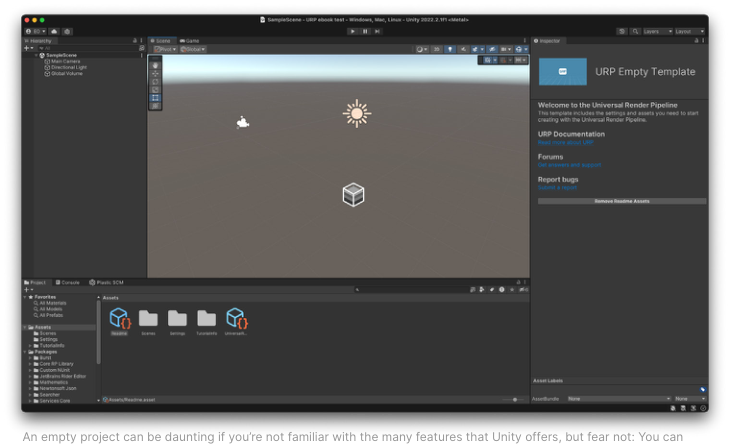
\includegraphics[width=0.78\linewidth]
  {../buku_ajar/chapters/12/figures/editor-unity.png}
\end{frame}

\begin{frame}{Panel dan Pertanyaan yang Dijawabnya}
\begin{itemize}
  \item \textbf{\emph{Hierarchy}} (kiri atas) --- daftar seluruh benda pada
        scene yang sedang dibuka, beserta hubungan kekeluargaannya. Menjawab
        ``benda apa saja yang ada di sini?''.
  \item \textbf{\emph{Scene}} (tengah, terluas) --- menampilkan scene dari
        sudut pandang perancang; benda dipindahkan dan diatur dengan
        menunjuknya langsung. Menjawab ``bagaimana susunan ruangnya?''.
  \item \textbf{\emph{Inspector}} (kanan) --- seluruh komponen benda yang
        sedang dipilih, beserta nilai setiap pengaturannya. Menjawab ``benda
        ini tersusun atas apa?''.
  \item \textbf{\emph{Project window}} (bawah) --- seluruh berkas project:
        scene, script, gambar, bunyi, dan aset lain. Menjawab ``berkas apa saja
        yang dimiliki project ini?''.
\end{itemize}
\vspace{0.12cm}
\begin{kotak}
Empat panel itu menjawab empat pertanyaan berbeda. Kebiasaan yang menghemat
waktu: pastikan panel mana yang sedang aktif sebelum menekan tombol, sebab
sebagian besar tombol pintas Unity bergantung pada panel aktif.
\end{kotak}
\end{frame}

\begin{frame}{Dua Daftar yang Mirip, tetapi Berbeda}
\begin{itemize}
  \item \textbf{\emph{Hierarchy}} memuat benda yang ada \textbf{di dalam scene
        yang sedang dibuka}.
  \item \textbf{\emph{Project window}} memuat \textbf{seluruh berkas} yang
        dimiliki project, termasuk scene lain yang belum dibuka.
  \item Akibatnya, sebuah berkas scene tidak tampak pada Hierarchy, dan sebuah
        benda di dalam scene tidak tampak pada Project window.
  \item \textbf{\emph{Game}} menampilkan scene dari sudut pandang kamera
        permainan, yaitu apa yang akan dilihat pemain.
  \item \textbf{\emph{Console}} menampilkan pesan \texttt{Debug.Log},
        peringatan, dan kesalahan; panel ini menggantikan terminal pada blok
        Python.
\end{itemize}
\vspace{0.12cm}
\begin{kiat}
Susunan panel dapat diubah dengan menggeser judulnya, dan susunan itu disimpan
di dalam project. Untuk keperluan pembelajaran, susunan bawaan sudah memadai.
\end{kiat}
\end{frame}

% ========================================================= bagian 3
\section{GameObject dan Komponen}
\sectionframe{03}{GameObject dan Komponen}
  {Wadah kosong yang menjadi berguna karena komponen yang menempel}

\begin{frame}{Benda Kosong yang Disusun dari Bagian}
\awalan{Sebuah GameObject pada dasarnya adalah wadah kosong: tidak bergambar,
tidak berbentuk, dan tidak melakukan apa pun.}
\begin{itemize}
  \item Yang membuatnya berguna adalah \emph{komponen} yang menempel padanya.
  \item \textbf{\emph{Transform}} --- memuat letak, putaran, dan ukuran benda.
        Komponen ini wajib ada pada setiap GameObject.
  \item \textbf{\emph{Mesh Renderer}} atau \textbf{\emph{Sprite Renderer}} ---
        menentukan bentuk atau gambar yang ditampilkan.
  \item \textbf{\emph{Collider}} --- menentukan bentuk batas benda untuk
        keperluan tabrakan.
  \item Komponen lain ditambahkan sesuai keperluan: \emph{Rigidbody} untuk
        benda yang mengikuti fisika, \emph{AudioSource} untuk benda yang
        bersuara, atau script C\# yang Anda tulis sendiri.
\end{itemize}
\vspace{0.14cm}
\begin{kotak}
Skrip yang Anda tulis pun berupa komponen. Satu skrip yang sama dapat
ditempelkan pada banyak benda, dan masing-masing menjalankannya sendiri dengan
nilainya sendiri. Inilah padanan kelas dan objek pada blok Python, tetapi
dengan cara yang berbeda.
\end{kotak}
\end{frame}

\begin{frame}{Dua Cara Menyusun Benda}
\begin{columns}[T,onlytextwidth]
  \begin{column}{0.48\textwidth}
    \begin{block}{Pada Pygame}
      \begin{itemize}
        \item Benda adalah objek dari kelas yang Anda tulis.
        \item Seluruh sifat dan perilakunya ditentukan oleh kelas itu.
        \item Benda yang berbeda perilakunya menuntut kelas yang berbeda.
      \end{itemize}
    \end{block}
  \end{column}
  \begin{column}{0.48\textwidth}
    \begin{exampleblock}{Pada Unity}
      \begin{itemize}
        \item Benda adalah wadah yang diisi komponen.
        \item Perilakunya ditentukan oleh komponen yang menempel.
        \item Benda yang berbeda perilakunya cukup diberi komponen berbeda.
      \end{itemize}
    \end{exampleblock}
  \end{column}
\end{columns}
\vspace{0.18cm}
\begin{itemize}
  \item Menambahkan kemampuan tidak menuntut perubahan kode, melainkan cukup
        dengan menempelkan komponen.
  \item Sebuah benda menjadi benda yang mengikuti fisika hanya dengan
        menambahkan Rigidbody, tanpa menyentuh satu baris kode yang sudah ada.
\end{itemize}
\vspace{0.10cm}
\begin{kotak}
Keduanya bertujuan sama, yaitu menyatukan data dan perilaku. Yang berbeda
adalah caranya: warisan kelas pada Python, penyusunan komponen pada Unity.
\end{kotak}
\end{frame}

\begin{frame}{Mengubah Pengaturan pada Inspector}
\awalan{Setiap komponen memiliki pengaturan, dan seluruhnya ditampilkan pada
Inspector. Nilainya diubah dengan mengetikkan angka atau menggeser penunjuk
sambil menekan tetikus.}
\begin{enumerate}
  \item \textbf{Nilai yang diubah ketika scene sedang berjalan tidak
        tersimpan.} Unity memisahkan nilai saat berjalan dari nilai tersimpan,
        sehingga percobaan tidak merusak susunan; nilainya dikembalikan ketika
        Anda berhenti menjalankan scene.
  \item \textbf{Pengaturan pada Inspector berasal dari kode Anda.} Perubahan
        pada nilai publik di dalam skrip tampak pada panel itu, dan nilai yang
        Anda ubah pada panel menimpa nilai bawaan pada skrip.
\end{enumerate}
\vspace{0.14cm}
\begin{kiat}
Berikan nilai bawaan yang masuk akal pada skrip Anda, sehingga benda yang baru
ditempeli langsung berperilaku wajar tanpa perlu diatur. Cara itu menghemat
waktu ketika skrip yang sama ditempelkan pada banyak benda.
\end{kiat}
\end{frame}

% ========================================================= bagian 4
\section{Scene, Project, dan Penyimpanan}
\sectionframe{04}{Scene, Project, dan Penyimpanan}
  {Satu tingkat permainan yang disimpan sebagai berkas}

\begin{frame}{Scene sebagai Satu Level}
\begin{itemize}
  \item Sebuah \emph{scene} adalah satu tingkat permainan, yaitu kumpulan
        benda beserta seluruh pengaturannya.
  \item Sebuah permainan dapat tersusun atas beberapa scene, misalnya satu
        scene untuk menu utama dan satu scene untuk setiap tingkat permainan.
  \item \textbf{Pada Pygame}, padanan scene adalah keadaan yang Anda susun
        sendiri di dalam kode: daftar objek, posisi awalnya, dan pengaturannya.
  \item \textbf{Pada Unity}, seluruh keadaan itu disimpan sebagai berkas,
        sehingga dapat dibuka, disunting, dan dijalankan tanpa menulis kode.
\end{itemize}
\vspace{0.14cm}
\begin{kotak}
Penyuntingan level yang pada blok Python dilakukan dengan mengubah kode kini
berpindah ke penyunting visual. Yang tetap menjadi pekerjaan Anda adalah
menentukan susunan ruang yang menghasilkan pengalaman bermain yang baik.
\end{kotak}
\end{frame}

\begin{frame}{Struktur Berkas Project}
\awalan{Setiap project Unity memiliki struktur folder yang tetap. Tiga di
antaranya perlu Anda ketahui.}
\begin{itemize}
  \item \texttt{Assets} --- seluruh berkas yang Anda buat dan impor: scene,
        script, gambar, bunyi, dan aset lain. Folder inilah yang disimpan pada
        repositori Git.
  \item \texttt{Library} --- berkas sementara hasil pengolahan Unity. Dapat
        dibangun ulang dan \textbf{tidak boleh} disimpan pada repositori,
        sebab ukurannya besar dan isinya berbeda pada setiap komputer.
  \item \texttt{ProjectSettings} --- pengaturan project, misalnya nama
        project, ukuran layar, dan scene mana yang dijalankan lebih dahulu.
\end{itemize}
\vspace{0.14cm}
\begin{peringatan}
Kebiasaan \texttt{.gitignore} dari blok Python tetap berlaku dan bahkan lebih
penting: daftarkan \texttt{Library}, \texttt{Temp}, \texttt{Obj}, dan
\texttt{Build}, sedangkan \texttt{Assets} dan \texttt{ProjectSettings} harus
disimpan. Folder \texttt{Library} dapat berukuran beberapa gigabita.
\end{peringatan}
\end{frame}

\begin{frame}{Menyimpan Pekerjaan}
\awalan{Unity menyimpan scene tidak secara otomatis, sehingga penyimpanan perlu
dilakukan dengan sengaja. Dua hal perlu dibedakan.}
\begin{itemize}
  \item \textbf{Menyimpan scene} menyimpan susunan benda beserta pengaturannya.
        Perintahnya tersedia pada menu \emph{File}.
  \item \textbf{Menyimpan script} menyimpan kode Anda. Berkas skrip disimpan
        oleh penyunting kode yang Anda pakai, bukan oleh Unity, dan Unity
        memuat ulang skripnya ketika Anda kembali ke jendelanya.
  \item Karena itu, perubahan kode yang belum disimpan tidak akan terlihat
        walaupun scene dijalankan berulang kali.
\end{itemize}
\vspace{0.16cm}
\begin{kiat}
Urutan yang menghemat waktu: simpan script lebih dahulu melalui penyunting
kode, baru simpan scene melalui Unity, lalu tekan tombol jalankan. Urutan itu
menghindarkan Anda menjalankan scene dengan skrip versi lama.
\end{kiat}
\end{frame}

% ========================================================= bagian 5
\section{Skrip C\# Pertama}
\sectionframe{05}{Skrip C\# Pertama}
  {Fungsi yang dipanggil mesin, bukan siklus yang Anda tulis}

\begin{frame}{Fungsi yang Dipanggil Mesin}
\awalan{Skrip belum berpengaruh sebelum ditempelkan pada sebuah GameObject:
seret berkasnya dari Project window, atau pakai \emph{Add Component} pada
Inspector. Skrip ini tidak memuat perulangan \texttt{while} dan tidak
memanggil gambar.}
{\scriptsize
\renewcommand{\arraystretch}{1.08}
\begin{tabularx}{\textwidth}{@{}>{\raggedright\arraybackslash}p{2.3cm}
    >{\raggedright\arraybackslash}p{3.5cm}
    >{\raggedright\arraybackslash}X@{}}
\toprule
\textbf{Fungsi} & \textbf{Kapan dipanggil} & \textbf{Dipakai untuk} \\
\midrule
\texttt{Awake} & Sekali, ketika benda dibuat &
  Menyiapkan rujukan ke komponen lain, termasuk yang tidak bergantung pada
  benda lain. \\
\addlinespace
\texttt{Start} & Sekali, sebelum bingkai pertama &
  Menyiapkan nilai awal yang bergantung pada benda lain, yang belum tentu siap
  ketika \texttt{Awake} dijalankan. \\
\addlinespace
\texttt{Update} & Sekali setiap bingkai &
  Menangani masukan dan hal yang mengikuti lama bingkai; padanan tahap
  pembaruan pada Bab IV. \\
\addlinespace
\texttt{FixedUpdate} & Berkala, dengan selang tetap &
  Menangani perhitungan fisika; padanan \emph{fixed timestep} pada Bab II. \\
\addlinespace
\texttt{OnDisable} & Ketika skrip dimatikan &
  Membereskan pekerjaan, misalnya menyimpan keadaan atau menutup berkas. \\
\bottomrule
\end{tabularx}}
\vspace{0.10cm}
{\footnotesize\color{ubMuted}Urutan itu ditentukan mesin, bukan kode Anda. Tugas
Anda adalah meletakkan pekerjaan pada fungsi yang tepat.}
\end{frame}

\begin{frame}[fragile]{Skrip Pertama: Start dan Update}
\lstinputlisting[language=CSharp,firstline=18,lastline=28,firstnumber=18]
  {../buku_ajar/code/unity/ch12_skrip_pertama.cs}
\kodejelas{\texttt{Start} dipanggil sekali sebelum bingkai pertama: posisi awal
disimpan dan dicatat. \texttt{Update} dipanggil setiap bingkai, dan selang
waktu satu bingkai disediakan mesin melalui \texttt{Time.deltaTime}.}
\end{frame}

\begin{frame}[fragile]{Gerak, Normalisasi, dan Selang Waktu}
\lstinputlisting[language=CSharp,firstline=30,lastline=43,firstnumber=30]
  {../buku_ajar/code/unity/ch12_skrip_pertama.cs}
\kodejelas{Arah dari tombol panah dinormalkan lebih dahulu, lalu dikalikan
kecepatan dan \texttt{deltaTime}; urutannya sama dengan Bab V. Tanpa
normalisasi, benda bergerak lebih cepat ketika menempuh arah diagonal.
\texttt{Rotate} memakai \texttt{turnSpeed * deltaTime} agar putaran tidak
bergantung laju bingkai.}
\end{frame}

% ========================================================= bagian 6
\section{Padanan Konsep dengan Pygame}
\sectionframe{06}{Padanan Konsep dengan Pygame}
  {Seluruh konsep tetap berlaku; yang berubah hanyalah nama dan cara memakainya}

\begin{frame}{Padanan Konsep Pygame dan Unity (1)}
\awalan{Blok Python tidak menjadi pekerjaan yang sia-sia: konsepnya tetap
berlaku, dan tabel ini memuat padanannya.}
{\scriptsize
\renewcommand{\arraystretch}{1.06}
\begin{tabularx}{\textwidth}{@{}>{\raggedright\arraybackslash}p{3.0cm}
    >{\raggedright\arraybackslash}p{4.4cm}
    >{\raggedright\arraybackslash}X@{}}
\toprule
\textbf{Konsep} & \textbf{Pada Pygame} & \textbf{Pada Unity} \\
\midrule
Siklus permainan & Perulangan yang Anda tulis (Bab IV) &
  Dijalankan mesin; Anda mengisi fungsi \texttt{Update}. \\
\addlinespace
Selang waktu & \texttt{delta\_seconds} hasil \texttt{clock.tick()} &
  \texttt{Time.deltaTime}. \\
\addlinespace
Keadaan benda & Variabel pada objek Python &
  Nilai \texttt{transform.position}, \texttt{transform.rotation}, dan peubah
  pada skrip. \\
\addlinespace
Gambar benda & \texttt{sprite.image} &
  Komponen \emph{Sprite Renderer} beserta aset gambarnya. \\
\addlinespace
Persegi pembatas & \texttt{sprite.rect} &
  \emph{Collider} beserta ukurannya. \\
\addlinespace
Gerak & \texttt{position += velocity * dt} (Bab V) &
  \texttt{transform.position += direction * speed * Time.deltaTime}. \\
\bottomrule
\end{tabularx}}
\end{frame}

\begin{frame}{Padanan Konsep Pygame dan Unity (2)}
{\scriptsize
\renewcommand{\arraystretch}{1.06}
\begin{tabularx}{\textwidth}{@{}>{\raggedright\arraybackslash}p{3.0cm}
    >{\raggedright\arraybackslash}p{4.4cm}
    >{\raggedright\arraybackslash}X@{}}
\toprule
\textbf{Konsep} & \textbf{Pada Pygame} & \textbf{Pada Unity} \\
\midrule
Fisika & Perhitungan sendiri (Bab VI) &
  Komponen \emph{Rigidbody}. \\
\addlinespace
Tabrakan & \texttt{spritecollide} dan penyelesaian per sumbu (Bab VII) &
  Diperiksa mesin dan dilaporkan sebagai peristiwa. \\
\addlinespace
Kelas benda & Kelas turunan \texttt{pygame.sprite.Sprite} (Bab VII) &
  \emph{GameObject} beserta komponennya. \\
\addlinespace
Wadah benda & \texttt{pygame.sprite.Group} &
  Daftar pada \emph{Hierarchy} atau kumpulan pada skrip. \\
\addlinespace
Tingkat permainan & Keadaan yang disusun di dalam kode &
  \emph{Scene}. \\
\addlinespace
Keluaran pesan & \texttt{print} pada terminal &
  \texttt{Debug.Log} pada panel \emph{Console}. \\
\bottomrule
\end{tabularx}}
\vspace{0.10cm}
{\footnotesize\color{ubMuted}Baris yang paling banyak berubah adalah baris
tentang \textbf{siapa yang mengerjakan}. Siklus tidak ditulis lagi; tabrakan
diperiksa mesin, tetapi penyelesaiannya tetap tanggung jawab Anda; kelas benda
diganti wadah komponen.}
\end{frame}

\begin{frame}{Konsep yang Tetap Sama Persis}
\awalan{Pada kedua perkakas, beberapa konsep tidak berubah sama sekali. Inilah
bekal terpenting dari blok Python.}
\begin{itemize}
  \item \textbf{Kecepatan dinyatakan dalam satuan per detik} dan dikalikan
        selang waktu. \texttt{Time.deltaTime} menggantikan
        \texttt{delta\_seconds}, tetapi perannya sama persis.
  \item \textbf{Arah dinormalkan sebelum dikalikan kecepatan}, agar gerak
        diagonal tidak lebih cepat.
  \item \textbf{Posisi sebenarnya disimpan sebagai pecahan}, sedangkan yang
        dipakai memeriksa tabrakan berupa bilangan bulat. Pada Unity, keduanya
        disediakan mesin.
  \item \textbf{Mendeteksi tabrakan dan menyelesaikannya adalah dua pekerjaan
        berbeda.} Yang pertama dapat diserahkan kepada mesin; yang kedua tidak.
  \item \textbf{Perhitungan yang mahal tetapi tidak mendesak sebaiknya
        disebar}, bukan dijalankan setiap bingkai (Bab XI).
\end{itemize}
\vspace{0.12cm}
\begin{kotak}
Kelima butir itu tidak dapat dipelajari dari panduan Unity mana pun, sebab
panduan membahas \textbf{cara memakai} Unity, bukan \textbf{cara kerja}
permainan. Pengetahuan itulah yang Anda peroleh dengan menulis seluruh
mekanismenya sendiri pada blok Python.
\end{kotak}
\end{frame}

% --------------------------------------------------------- aktivitas
\begin{frame}{Aktivitas di Kelas \textperiodcentered\ Praktikum 09}
\awalan{Pengalaman belajar minggu 11 pada RPS. Berkas tugas bernomor 09 karena
mengikuti urutan tugas, sedangkan minggu kuliahnya 11.}
\begin{enumerate}
  \item Pasang Unity Hub, lalu satu versi Unity LTS beserta modul dukungan 2D;
        catat nomor versinya pada lembar kerja.
  \item Buat \emph{project} 2D melalui Unity Hub, lalu tentukan panel mana yang
        Hierarchy, Scene, Inspector, dan Project window.
  \item Kenali scene bawaannya: tentukan kamera, pencahayaan, dan objek
        primitif; geser objek itu pada panel Scene dan amati nilai pada
        Inspector.
  \item Tambahkan tiga objek primitif berbeda (kubus, bola, silinder), susun
        berjajar, lalu atur warnanya agar berbeda-beda.
  \item Ketik ulang \texttt{ch12\_skrip\_pertama.cs} ke folder
        \texttt{Scripts}, tempelkan pada salah satu objek, jalankan scene, dan
        amati pesan pada Console.
  \item Simpan scene dan project, periksa isi folder \texttt{Assets}, susun
        tabel padanan dengan kata-kata sendiri, dan simpan ke repositori Git
        dengan \texttt{.gitignore} yang tepat.
\end{enumerate}
\vspace{0.08cm}
{\footnotesize\color{ubAccent}\itshape Rincian lengkap: Praktikum 09 pada Bab
XII buku ajar. Kumpulkan melalui repositori Git pribadi.}
\end{frame}

% --------------------------------------------------------- rangkuman
\begin{frame}{Rangkuman}
\begin{itemize}
  \item Mesin permainan mengambil alih siklus, fisika, deteksi tabrakan,
        penayangan, dan penyuntingan level; kode Anda mengisi tahap yang
        disediakan mesin.
  \item Unity dipasang melalui Unity Hub dan Unity Editor; versi LTS dipilih
        karena lebih stabil dan lebih banyak dipakai.
  \item Empat panel utama: Hierarchy memuat benda di dalam scene, Scene
        menampilkan susunan ruangnya, Inspector menampilkan komponen benda
        terpilih, dan Project window memuat seluruh berkas project.
  \item GameObject adalah wadah kosong yang berguna karena komponennya;
        Transform wajib ada, komponen lain ditambahkan sesuai keperluan.
  \item Fungsi skrip dipanggil mesin: Awake dan Start sekali di awal, Update
        setiap bingkai, FixedUpdate dengan selang tetap, OnDisable saat
        dimatikan.
  \item Scene adalah satu tingkat permainan yang disimpan sebagai berkas;
        Assets dan ProjectSettings disimpan, Library tidak.
\end{itemize}
\end{frame}

% --------------------------------------------------------- cek
\begin{frame}{Cek Pemahaman}
\begin{enumerate}
  \item Mengapa sebuah berkas scene tidak tampak pada Hierarchy, sedangkan
        benda di dalam scene tidak tampak pada Project window?
  \item Jelaskan gagasan penyusunan benda pada Unity, lalu bandingkan dengan
        cara menyusun benda pada Pygame.
  \item Kapan \texttt{Update} dan \texttt{FixedUpdate} dipanggil, dan mengapa
        keduanya dipisahkan?
\end{enumerate}
\vspace{0.35cm}
{\footnotesize\color{ubMuted}\itshape Jawab tanpa membuka catatan, lalu
bandingkan dengan pasangan di sebelah Anda.}
\end{frame}

% --------------------------------------------------------- penutup
\penutup{Tugas Praktikum 09}
  {Materi 11 menyusun level yang dapat dimainkan: \emph{tilemap} dan
   \emph{greyboxing}, \emph{Collider} dan \emph{Rigidbody}, serta script kontrol
   pemain pada \texttt{Update} dan \texttt{FixedUpdate}.}

\end{document}
